\section{Behandlingsmetoder}
\textit{I dette afsnit beskrives knæleddet og hvordan artrose påvirker dette med henblik på senere forståelse for hvordan behandlingsmetoderne for knæartrose fungerer. Non-invasive behandlingsmetoder undersøges for at bestemme effekten af disse, hvorefter udførelsen af en knæalloplastik og kriterierne for en succesfuld TKA-operation analyseres med henblik på at vurdere om operationsteknikken er årsag til, at patienter får kroniske postoperative smerter.}

\subsection{Knæleddet}
Knæleddet er et synovialt, sammensat led med en bevægelsesgrad fra 0 til 135$\degree$ for fleksion og 0 til 5$\degree$ for hyperekstension. Knæleddet er kroppens største led, og er således udsat for større mekaniske påvirkninger end noget andet led i kroppen. Hermed oplever knæleddet hyppigere end noget andet led patologiske forandringer. Knæleddet er sammensat af tre knogler; femur, tibia og patella. Disse er alle på slidfladerne beklædt med et tykt lag hyalinbrusk. Dette lag kan være op til syv millimeter tykt. Sammen med meniskerne, der fordeler trykket på en større overflade, er hyalinbrusken med til at mindske friktionen i leddet. \citep{Moeller2001}

\subsection{Knæartrose}
Knæartrose opdeles i en primær og sekundær tilstand. Den primære artrose betegner artrose, der opstår som følge af ikke-udefrakommende årsager, herunder genetik og aldring. Den sekundære artrose forårsages af tidligere skader, inflammation, overvægt og traume. Knæartrose er en tilstand, hvis hyppigste symptomer er smerter, nedsat mobilitet samt fejlstilling af leddet hos den påvirkede. Smerterne forekommer i forskellig grad fra igangsættende smerte til konstant smerte. Symptomerne forværres som lidelsen udvikler sig. \citep{Lind2016b}

\begin{figure}[H] 
\begin{center}
\includegraphics[width=0.6\textwidth]{figures/bProblemanalyse/Artose_knae}
\end{center}
\caption{Figuren viser, hvad der sker i knæleddet, når det undergår patologiske forandringer ved knæartrose. Det ses af figuren til højre, at strukturne i knæet forandrer sig. Det fremgår, at bruskelementerne, ved infektion, slid eller traume, kan blive beskadiget, hvilket vil eksponere knoglen og føre til smerte og funktionsnedsættelse. På figuren til højre ses ligeledes osteofytter. \citep{schroder} \citep{adobe}} 
\label{fig:tka_implant} 
\end{figure}

\subsection{Non-invasiv behandling}
Artrose kan ikke helbredes og non-invasive behandlingsmetoder vil derfor fortrinsvis søge at smertelindre samt forbedre funktionen af knæet \citep{brostrom2012}. En essentiel del af behandlingen, består i at informere og uddanne patienten, give indsigt i sygdommen samt aktiv at indrage patienten i behandlingsforløbet. Det ønskes eksempelvis at patienten forstår vigtigheden af et vægttab, såfremt dette er nødvendigt. \citep{brostrom2012}
Ved behandling af artrose benyttes ligeledes medicin  til smertelindring samt forbedring af funktion. De benyttede præparater er paracetamol, men også NSAID præparater kan anvendes ved inflammation \citep{schroder}. Ved kraftige smertegener, hvor de primære præparater til behandling ikke har haft den ønskede effekt, kan opioider benyttes. \citep{brostrom2012}

I både nationale og internationale kliniske retningslinjer, er der bred konsensus om, at træning er af væsentlig betydning ved behandling af knæartrose \citep{brostrom2012}. Et studie med data fra over 4.000 patienter, foretaget af \citer{Syssorenskou} viste, at hverken graden af den radiologiske artrose eller smerteintensitet havde indvirkning på hvor stor effekt, der kunne forventes af træningsforløbet. Det blev fundet, at patienter med svær artrose oplevede samme smertereduktion, som patienter med let til moderat artros. Et studie af \citer{sorenskou} fandt evidens for, at smertelindringen ved træning var lige så stor som ved brug af NSAID'er og endnu større end ved brug af paracetamol. Træning har desuden, modsat medicinsk behandling,  ingen bivirkninger. \citep{sorenskou}
Et studie af \citer{newEngland} fulgte 100 forsøgspersoner, som var egnet til at få foretaget en TKA-operation, over et år. Den ene gruppe modtog non-invasiv behandling, som bestod af et træningsforløb, patientundervisning, indlægssåler og et eventuel vægtabsprogram. Den anden gruppe modtog kirurgisk behandling. Gruppen, der gennemgik kirurgisk behandling, havde en større smertelindring end gruppen, som kun modtog non-invasiv behandling. Dog havde gruppen, der modtog kirurgisk behandling, større risiko for at få komplikationer. Forsøget viste dog, at i gruppen som modtog non-invasiv behandling, fik cirka en tredjedel foretaget en TKA i løbet af forsøgsperioden. \citep{newEngland} 

%Dette kan muligvis betyde at et non-invasivt forløb kan være være med til udskyde et operativt indgreb. (\textbf{vi skal nok passe på med at konkludere noget her})

%\subsection{Knæartrose}
%
%Knæartrose også kaldet slidgigt i knæene, har mange årsager. Hvor af nogle er overvægt, arv, traume eller tungt arbejde. Arterose er karakteriseret ved ødelæggelse af ledbrusken med dertil hørende reaktioner i de tillæggende knogler og slimhinder. Symptomerne på knæartrose er smerte, funktionstab og fejlstilling, hvilket besværliggøre hverdagen. 
%Ved knæartrose er sidste behandlings skridt kirurgi, afhængig af graden af traumet er forskellige kirurgiske indgreb en mulighed. [Nationale retningslinjer] 

\subsection{Kirurgisk behandling}
Som kirugisk behandling for knæartrose foretages oftest en alloplastik. Alloplastik er et operativt indgreb der har til formål helt eller delvist at udskifte knæleddet med specialdesignede metal- og plastkomponenter. Der findes to former for alloplastikker; udskiftning af hele knæleddet (TKA) eller udskiftning af en del af knæleddet (UKA). \citep{brostrom2012}

\begin{figure}[H] 
\begin{center}
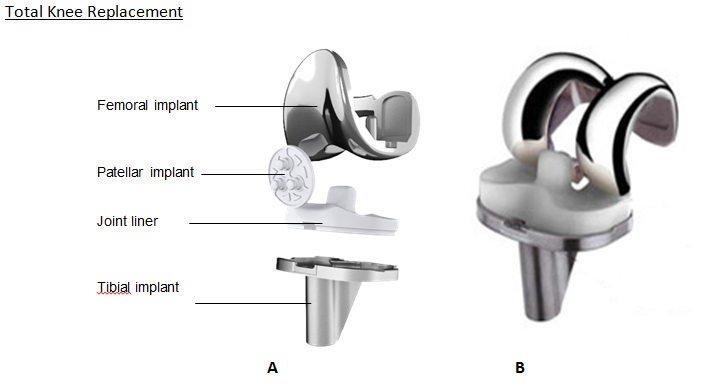
\includegraphics[width=0.7\textwidth]{figures/tka_implant}
\end{center}
\caption{En TKA består af fire komponenter; et femoralt, patella- og tibialt implantat samt et plastiklag, der placeres mellem det femorale og tibiale implantat og mindsker friktionen. Udformningen af komponenterne gør det muligt at efterligne knæleddets naturlige bevægelse. \citep{robodoc2016}} 
\label{fig:tka_implant} 
\end{figure}

Under alloplastik operationen ligger patienten  på operationsbordet med knæet i en flekteret position. Et snit lægges over patella, hvorefter denne og senerne i leddet eleveres og blotter knæleddet. Hermed får kirurgen adgang til bruskfladerne på femur og tibia. Kirurgen fjerner  det ødelagte brusk og en del af knoglen ved hjælp af en guideblok, der skrues ind i femur og sikrer præcis fjernelse af den ønskede mængde væv. Dette gentages på tibia, hvorved der skabes plads til implantaterne. Midlertidige implantater indsættes for at sikre bevægelsesfriheden er bevaret og testes ved ekstension af knæet. Når kirurgen er tilfreds med resultatet, bores guidehuller i henholdsvis femur, tibia og patella til fastmontering af de permanente implantater. Fastmonteringen sker ved at dække implantatet og monteringsstedet i bencement, der limer proteserne fast til den eksisterende knoglestruktur. Herefter sikres igen, at bevægelsesgraden er bibeholdt, førend indsnittet lukkes og operationen er fuldendt. En TKA-operation varer typisk omkring én time, hvorefter patienten kan støtte på benet den følgende dag. Efter operationen følger et rehabiliteringsforløb for at støtte og styrke muskulaturen omkring knæet. \citep{Sanna2013} \citep{tka-technique}

Ifølge Sundhedsstyrelsens vurdering er knæalloplastik en effektiv behandling til at mindske smerte, øge funktion og derved forøge patientens livskvalitet. Holdbarheden af knæimplantaterne vurderes ud fra antallet af implantater, der er vurderet udskiftet efter 10 år, hvor det er påvist, at 90 til 95\%~ af implantaterne ikke er revideret. Det er ikke muligt at vurdere holdbarheden af den enkelte protese, da flertallet af patienterne dør med et velfungerende implantat. \citep{brostrom2012}

\subsubsection{Kriterier for veludført TKA-operation}\label{tek_succes}
Kriterierne for succesfuld kirurgisk behandling af knæartrose er ifølge Styringsgruppen for Dansk Knæalloplastikregister (DKA) opdelt i fem kriterier. \citep{aarsrapport2016} Disse kriterier er opgivet i tabel \ref{succeskriterier}, hvor standdard og landsgennemsnit for Danmark ligeledes er opgivet. 
%, som alle bygger revisionsraten. Altså patienter som har behov for en yderligere knæ operation.

\begin{table}[]
\centering
\resizebox{\textwidth}{!}{%
\begin{tabular}{ccc}
\rowcolor[HTML]{C0C0C0} 
                                                                                                                                        & \begin{tabular}[c]{@{}c@{}}Standard\\{[}maximale \%{]}\end{tabular} & Landsgennemsnit (Spredning) {[}\%{]} \\ \hline
Andel af patienter med primær TKA på baggrund af primær artrose, \\ som, uanset diagnose, genindlægges indenfor 30 dage efter udskrivning. & 10                                                                                  & \begin{tabular}[c]{@{}c@{}}7,3 \\ (5,8 til 9,5)\end{tabular} \\
Andel af patienter med primær TKA der er revideret indenfor et år.                                                                      & 3                                                                                   & \begin{tabular}[c]{@{}c@{}}1,8 \\ (0,8 til 2,4)\end{tabular} \\
Andel af patienter med primær TKA der er revideret indenfor to år.                                                                      & 5                                                                                   & \begin{tabular}[c]{@{}c@{}}3,3\\ (1,7 til 4,8)\end{tabular}  \\
Andel af patienter med primær TKA der er revideret indenfor fem år.                                                                     & 8                                                                                   & \begin{tabular}[c]{@{}c@{}}6\\ (4,2 til 6,7)\end{tabular}    \\
Andel af patienter, der dør indenfor 90 dage efter primær TKA.                                                                          & 1                                                                                   & \begin{tabular}[c]{@{}c@{}}0,4\\ (0 til 0,7)\end{tabular}    \\ \hline
\end{tabular}%
}
\caption{Tabellen viser succeskriterierne for knæalloplastikoperationer med en standardiseret grænse sammenholdt med landsgennemsnittet. Spredning er indikeret i parentes. Tabellen er modificeret fra \cite{aarsrapport2016}}
\label{succeskriterier}
\end{table}

Det fremgår af \tabref{succeskriterier}, at der, i hele Danmark, udføres knæalloplastikker som alle overholder retningslinjerne for behandlingskvaliteten \citep{aarsrapport2016}. 
På trods af at alle operationer overholder de opstillede kriterier, har en betydelig procentdel af patienterne kroniske postoperative smerter.  \citep{Bourne2010} Hermed opfyldes succeskriterierne opstillet af DKA, hvormed næsten alle knæalloplastikker kan anses som at være succesfulde. Dette er dog modstridende med andelen af operationer der er tilfredsstillende ud fra et patientsynspunkt. Det er således væsentligt at identificere eventuelle præoperative risikofaktorer for udvikling af kroniske smerter efter en TKA-operation.  

Et studie af \citer{Lewis2015} har undersøgt prædikatorer associeret med kroniske postoperative smerter ved TKA-operationer. Det blev fundet, at katastrofetænkning, mentalt helbred, smerte forud for operationen og smerte andre steder var de største årsager til postoperative smerter mere end tre måneder efter en TKA-operation. 



%
%(1) http://www.robodoc.com/patient_about_faqs.html
%
%(2) https://www.youtube.com/watch?v=tKji04oFGdU

% (3) http://www.ortopaedi.dk/fileadmin/Guidelines/Referenceprogrammer/Osteotomi_og_TKA.pdf

	%(4) Surgical approaches in total knee arthroplasty.
	
%	(5) tka-technique
%
%(79) Dahl AW, Toksvig-Larsen S, Roos EM. A 2-year prospective study of patient- relevant outcomes in patients operated on for knee osteoarthritis with tibial osteot- omy. BMC Musculoskeletal Disorders 2005;6(1):18. Er lagt på mendlay
%(80) Hoell S, Suttmoeller J, Stoll V, Fuchs S, Gosheger G. The high tibial osteoto- my, open versus closed wedge, a comparison of methods in 108 patients. Arch Or- thop Trauma Surg 2005;125(9):638-643. Er lagt på mendelay

%Når de non-kirurgiske behandlingsmuligheder ikke har kunne løse patienten fra smerter, er kirurgi det næste skridt i behandlingsforløbet. Der findes flere behandlingsmuligheder inden for kirurgiskbehandling af knæartrose, dog med TKA som den endelige udvej. %Valget af operation og typen af den afhænger af flere faktorer, blandt andet patients alder, aktivitetsniveau og hvor fremskreden artrosen er.


%\subsubsection{Osteotomi}
%Ved degenerative forandringer i knæleddet, grundet primær eller postttrumatisk knæledsarterose, kan patienter opleve belastningsreleaterede smerter, hvilket blandt andet kan skyldes fejlstilling. Osteotomi har tilformål at afhjælpe den mekaniske belastning i det berørte område, for derved at afhjælpe smerterne. Ved osteotomi fjernes der oftest en kile af tibia-knoglen og det resterende knogle sikres med skruer og metal plader. Proceduren ændre knæets mekaniske akse, hvilket vil ændre belastningen af de degenererede områder. \citep{Osteotomi_og_TKA} Ved yngre (<50år) og aktive patienter vil der være større sandsynelighed for at tilbyde osteotomi frem for den mere invasive TKA, derfor anbefales osteotomi af sundhedstyrelsen til behandling af mildere former for artrose med fejlstilling \citep{Osteotomi_og_TKA} \citep{brostrom2012}. Behandlingen ses som en midlertidig behandling der kan udskyde behovet for TKA. Ifølge et kohordestudie kan der forventes en smertelindring hos 80\%~ af patienterne der får udført osteotomi. \textbf{rigtige kilder tak!(79)(80)} Ifølge \cite{brostrom2012} må det forventes at 30 til 50\%~ af patienterne der får foretaget en osteotomi, senere vil få behov for en alloplastik operation. \citep{brostrom2012} Tilbagevendende smerter korreleres til tab af korrektionen, samt progression af artrosen. Får patienten således svære smerte igen, kan en TKA komme til overvejelse \citep{Osteotomi_og_TKA}. 
% \textbf{Der er data på mere specifikke tilfredsheds undersøgelser, men ser ikke nogen trund til at medtage dem. }